\section{Implementação}

A expressão matemática, ou indivíduo, é representado por uma árvore composto de terminais e não terminais.

As folhas terminais são compostas pelos tipos \textbf{Constant} e \textbf{Variable}.

\begin{itemize}
	\item \textbf{Constant}, como o nome já explica, retorna uma constante.
	\item \textbf{Variable}, variável $X_i$ retornando o valor dado de entrada na dimensão $i$.
\end{itemize}

Nós não terminais é composto por operadores e funções.

\begin{itemize}
	\item \textbf{Operadores}
	\begin{itemize}
		\item \textbf{+}, soma.
		\item \textbf{-}, subtração.
		\item \textbf{x}, multiplicação.
		\item \textbf{/}, divisão.
	\end{itemize}
	\item \textbf{Funções}
	\begin{itemize}
		\item \textbf{Exp}, exponencial neperiano $e^x$.
		\item \textbf{Ln}, logaritmo neperiano $\ln x$.
		\item \textbf{Sin}, função trigonométrica $\sin x$.
		\item \textbf{Cos}, função trigonométrica $\cos x$.
	\end{itemize}
\end{itemize}

A divisão tem probabilidade menor de ser gerada para evitar funções mal comportadas com intuito de evitar a criação de expressões que ocasionam \textit{overfitting}. Em outras palavras as derivadas e-nésimas são limitadas.

\[N \le f^n(x) \le M\]

\subsection{Indivíduo}

Uma instância da expressão $\sin(e^{x_1}) + \cos(\ln(x_2 - 0.42))$ é mostrada na figura \ref{fig:indtree}. 

\begin{figure}
  \centering
  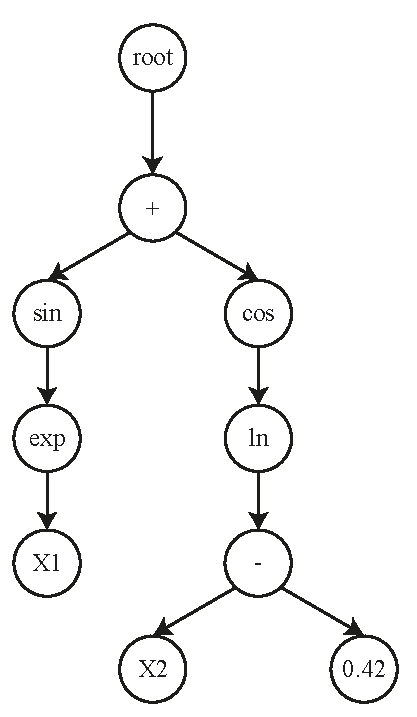
\includegraphics[width=0.25\textwidth]{pdf/expre.pdf}
  \caption{Representação do indivíduo através de uma árvore.}
  \label{fig:indtree}
\end{figure}

Cada sub-árvore possui um ID único, que é o SHA256 da string da expressão, para utilizar como identificador em armazenar cálculos de fitness ou identificar nós para efetuar cruzamento ou mutação.

Durante o período de treinamento, todas as fitness já calculadas são armazenadas em um dicionário para evitar cálculos subsequentes ou para identificar indivíduos repetidos.

Expressões que tiverem prefundidade alta, $\ge 7$, são penalizadas na fitness com $\infty$ para que evite crescimento exagerado dos indivíduos com objetivo de dispensar indivíduos esparsos.

\subsection{População Inicial}

A população inicial é gerada aleatóriamente sem nenhuma restrição ou tendência em criar um tipo de função especifica.

\subsection{Operadores Genéticos}

Os operadores genéticos utilizados são:

\begin{itemize}
	\item \textbf{Crossover}

	Escolhido dois indivíduos $I_{p1}$ e $I_{p2}$, é selecionado aleatóriamente um nó de cada um para se efetuar a troca, como ilustrado na figura \ref{fig:cross1}. Em seguida é feita a troca dos nós junto com os filhos delas, ilustrado na figura \ref{fig:cross2} gerando os indivíduos $I_{f1}$ e $I_{f2}$.

	\begin{figure}[H]
	  \centering
	  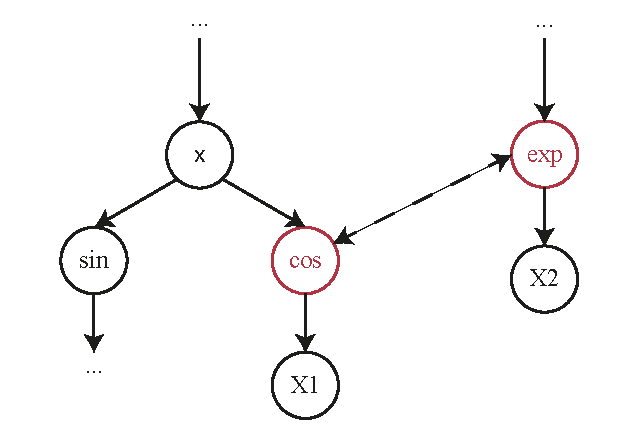
\includegraphics[width=0.3\textwidth]{pdf/cross_ex_1.pdf}
	  \caption{Seleção aleatória dos nós.}
	  \label{fig:cross1}
	\end{figure}

	\begin{figure}[H]
	  \centering
	  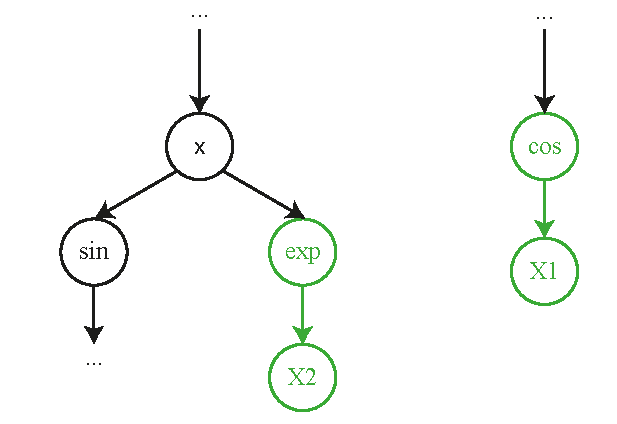
\includegraphics[width=0.3\textwidth]{pdf/cross_ex_2.pdf}
	  \caption{Seleção troca dos nós efetuada.}
	  \label{fig:cross2}
	\end{figure}

	Ao final, é feito uma operação de elitismo que é calculado as fitness de $I_{f1}, I_{f2}$ e comparado com os pais $I_{p1}$ e $I_{p2}$. São selecionado os dois melhores para a próxima geração.

	\[\textrm{crossover}(I_{p1}, I_{p2}) \rightarrow \textrm{2min\_fitness}(I_{p1}, I_{p2}, I_{f1}, I_{f2})\]

	\item \textbf{Mutation}

	De modo análogo ao crossover, dado um indivíduo $I_p$, seleciona-se aleatóriamente um nó da árvore \ref{fig:mut1}, elimina-se esta sub-árvore e em seguida se gera outra sub-árvore aleatóriamente \ref{fig:mut2} gerando o indivíduo filho $I_f$.

	\begin{figure}[H]
	  \centering
	  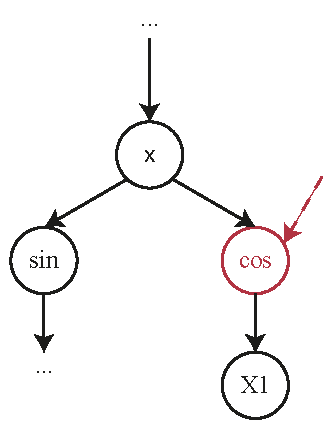
\includegraphics[width=0.25\textwidth]{pdf/mut_ex_1.pdf}
	  \caption{Seleção aleatória do nó.}
	  \label{fig:mut1}
	\end{figure}

	\begin{figure}[H]
	  \centering
	  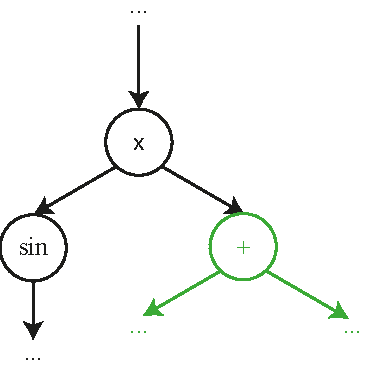
\includegraphics[width=0.25\textwidth]{pdf/mut_ex_2.pdf}
	  \caption{Geração da sub-árvore no nó removido.}
	  \label{fig:mut2}
	\end{figure}

	Ao final é comparado e passa-se o indíviduo com menor fitness para a próxima geração.

	\[\textrm{mutation}(I_p) \rightarrow \textrm{min\_fitness}(I_p, I_f)\]

	\item \textbf{Reproduction}

	Não é feito nenhuma modificação ao indivíduo e é repassado para a próxima geração.

\end{itemize}

As 3 operações são executadas iterativamente e probabilísticamente até que se complete os $n$ indivíduos. Em cada seleção, é feito um torneio em que se escolhe $k$ indivíduos aleatóriamente, que em seguida será feito as operações no melhor ou dois melhores do torneio.

A probabilidade do \textit{crossover} e \textit{mutation} são passados como parâmetros $p_b$ e $p_m$ respectivamente tal que $0 \le p_b, p_m \le 1$.

A probabilidade da reprodução é o complemento das duas probabilidades.

\begin{equation}
  \begin{array}{l}
    P(\textrm{reprodução}) = 1 - P(\textrm{crossover}) - P(\textrm{mutation}) \\ 
    P(\textrm{crossover}) + P(\textrm{mutation}) + P(\textrm{reprodução}) = 1
  \end{array}
\end{equation}



